\documentclass[a4paper, 12pt]{article}

\marginparwidth 0.5in 
\oddsidemargin 0.25in 
\evensidemargin 0.25in 
\marginparsep 0.25in
\topmargin 0.25in 
\textwidth 6in \textheight 8 in

\usepackage{multirow}
\usepackage{tabularx}
\usepackage{longtable}
\usepackage{tabu}
\usepackage{anyfontsize}
\usepackage{hyperref}
\usepackage{graphicx}
\usepackage{minted}
\usepackage{courier}

\begin{document}

\author{Aniket Shirke(150100012) \\Guide: Prof. Umesh Bellur}
\title{\textbf{ Simulator for IoT Analytics }}

\maketitle
\begin{figure}[ht]
    \begin{center}
        \includegraphics[scale=1]{iitbblack.jpg}
    \end{center}
\end{figure}
 
\begin{abstract}

\end{abstract}

\newpage
\tableofcontents
\newpage

\section{Introduction}

There has been an explosion in the deployment of IoT devices, generating enormous amounts of data in the form of fast-moving data streams. Typically this data is pushed up to a central server where either a classification or a prediction model can be trained and this method is not suitable for handling enormous amounts of data. Another concurrent trend has been the emergence of the Edge, having limited computational resources, as an alternative to reliance on Cloud resources. Rather than sending all data up to the Cloud, we can have a hierarchy of Edge centers that will train the model in a data distributed manner.

To obtain the cost vs accuracy analysis of a given model, we need a simulation environment where we can simulate different degrees of distribution and their effect on the cost of data transfer as well as on the accuracy of the model at Edge centers as learning progresses.  This will help us decide on a distribution strategy of the Edge devices. The objective of the Simulator: For a given data stream and available Edge devices with known computational constraints, compare the performance of a given deep neural network for multiple logical trees of Edge devices and suggest an optimal logical tree for that deep learning model.

The proceeding sections in the report describe the functionality of the Simulator, some important technical features and the results obtained using it.

\section{Simulator Functionality} 
Each Edge center at the lowest level, which we will refer to as a Worker, receives a subset of data closest to it and trains the model on the data it gets. Periodically these Worker nodes send their model parameters up to a Parameter Server (hosted at an Edge center) which merges the learning of the different edge centers and sends the merged model back to the lower level edge centers, i.e. Workers. In order not to overwhelm a Parameter Server with too many Worker nodes, there can be possibly multiple parameter servers for merging model parameters. The process of refining the model is therefore incremental and hierarchical. 

The Simulator treats the Parameter Server and the Worker as nodes in the learning tree. The Simulator starts of by initializing the root node of the learning tree first and then starting the corresponding children. A Worker node finishes its simulation after processing a specified number of windows of data. For a given internal node, the node stops simulating only after all children finish simulating. Thus, the Simulation starts in a top-down fashion and ends in a bottom-up manner with respect to the learning tree

We move on to the current functionality the Simulator performs to learn a given model.

\subsection{Worker}
A Worker node spawns two threads:
\begin{itemize}
    \item To run the training thread. For each window of data the Worker node processes, it:
    \begin{enumerate}
        \item Pulls the model from parent 
        \item Runs training algorithm as defined by the application
        \item Logs Statistics for the window
        \item Pushes new model to the parent 
    \end{enumerate}
    \item To run the RPC server for inter-node communication
\end{itemize}

\subsection{Parameter Server}
A Parameter Server spawns two threads:
\begin{itemize}
    \item To consume the gradients being obtained from child Worker nodes. For each merging of gradients, it:
    \begin{enumerate}
        \item Monitors the queue of acquired gradients from the child Worker nodes
        \item Pulls model from parent 
        \item Logs the accuracy of the model before merging gradients
        \item Modifies its own model using those gradients
        \item Logs the accuracy of the model after merging gradients
        \item Pushes new model to the parent (if it is not the root node)
    \end{enumerate}
    \item To run the RPC server for inter-node communication
\end{itemize}

The following statistic is recorded by the Worker node after processing every window:
\begin{itemize}
    \item Window ID: ID of the window of data processed
    \item Run time: Total time taken to process the window, calculated using \texttt{time.perf\textunderscore counter()} in python
    \item Process time: CPU time taken to process the window, calculated using \texttt{time.process\textunderscore time()} in python
    \item Memory usage: Memory usage recorded at the end of processing the window
    \item Accuracy: To analyse the spatial and temporal variation in accuracy, the model is evaluated against different test sensor data 
\end{itemize}

\section{Simulator Features}
To simulate real life scenarios, issues such as link delays, streaming data and resource constraints have been incorporated in the Simulator. This section elaborates on the Master Slave model - to automate execution of multiple experiments, Kafka integration for streaming data and Docker Containerization.

\subsection{Master Slave Model}
\begin{figure}[ht]
    \begin{center}
        \includegraphics[scale=0.5]{simulator_design.png}
    \end{center}
\end{figure}

\subsubsection{Motivation}
Training Deep neural networks takes considerable amount of time, sometimes even a few hours. In order to ease the execution of experiments, a Master-Slave model is proposed so that different experiments can be scheduled on a Master machine to collect simulation logs submitted by Slave machines.
\subsubsection{Design}
The Master and Slave machines are Linux servers. The Master starts an RPC server to receive logs about the simulation from the Slaves. It is assumed that the code required for running the nodes is present on the Slave machine. The Master reads the credentials of the Slaves from the configuration file, logs into the Slave machines and triggers nodes with the option to containerize the node. 

\subsection{Kafka Integration}
\begin{figure}[ht]
    \begin{center}
        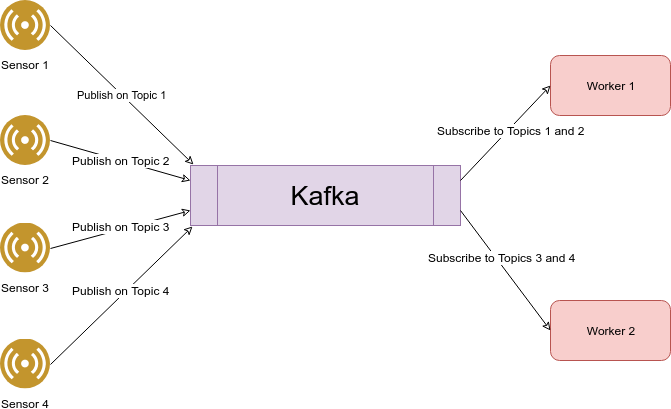
\includegraphics[scale=0.5]{kafka_integration.png}
    \end{center}
\end{figure}
\subsubsection{Motivation}
In real world scenario, there are sensors stream data to the Cloud after regular interval. It is expected that the Worker nodes running on the Edge receive data from sensors. To simulate this effect of streaming data from sensors on training the model, Kafka has been used to leverage its publish-subscribe model. 
\subsubsection{Design}
In the publish-subscribe messaging paradigm, publishers publish messages to a specific topic and subscribers consume messages related to the topic by subscribing to that topic. 

Every sensor is assumed to have a sensor ID. Here, the publishing entity is a sensor, which publishes data to the topic which is the same as its own sensor ID. The sensor is effectively a python script which reads the sensor data from a file and dumps it at a fixed data rate into a Kafka server.
In the configuration file, an array of sensors is assigned to each Worker node. Every Worker node then subscribes to the corresponding sensor ID and consumes data for training the model.

\subsection{Containerization}
\subsubsection{Motivation}
Edge devices have constraints on their resources, in terms of computational capability and memory usage. In order to simulate these effects, Docker has been used to impose resource constraints by containerizing code execution.
\subsubsection{Design}
Docker allows us to containerize our code in the form of an image, and multiple Docker containers can be created as an instantiation of a single image. Along these lines, a Docker image is initially created which contains the script for running Edge nodes. The node ID, node data (from the configuration) and the address of the Kafka server is passed as an environment variable.
The Master machine now logs into the Slave machine, specifies the number of cores and memory to be given and triggers a Docker containers.  

Docker specific design choices:
\begin{enumerate}
    \item \textbf{Networking}: The Docker container, in which the node runs, shares the networking stack with the host Slave machine.
    \item \textbf{Storage}: For testing the model accuracy, we need access to raw data files which contain the sensor data. If we include the data files in building the image, the image size will blow up to tens of Gigabytes. As a host Slave can support multiple Docker containers and to reduce the Docker image size, the sensor data is kept on the host's file system and the directory is bind to an empty directory of the Docker image.  
    \item \textbf{File reading}: In order to avoid reading the whole data file (few Gigabytes) into the memory of a running container (hundreds of Megabytes), an optimization has been done to sample data points from the file by seeking to lines arbitrarily.
\end{enumerate}

\subsection{Implementation}

\section{Running the Simulator}

\subsection{Configuration setup}
Every experiment has a corresponding configuration file in the form of yaml.
\begin{figure}[ht]
    \begin{center}
        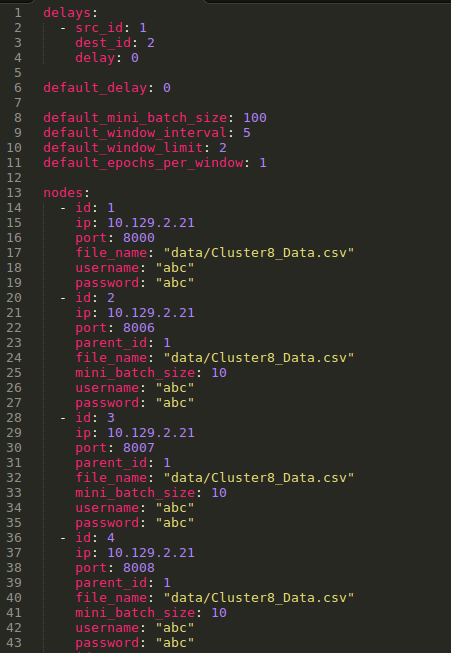
\includegraphics[scale=0.5]{config.png}
    \end{center}
\end{figure}

Common fields for configuration:
\begin{itemize}
    \item \texttt{delays}: Link delays between nodes specified pairwise
    \item \texttt{default\textunderscore delay}: Default link delay between nodes
    \item \texttt{default\textunderscore mini\textunderscore batch\textunderscore size}: Default mini batch size for training (Field depends on the algorithm used)
    \item \texttt{default\textunderscore window\textunderscore interval}: Default time interval for which data is collected by worker node
    \item \texttt{default\textunderscore window\textunderscore limit}: Default number of windows processed by worker during the experiment
    \item \texttt{default\textunderscore epochs\textunderscore per\textunderscore window}: Default number of epochs to run on training data collected in a window 
    \item \texttt{default\textunderscore kafka\textunderscore server}: Default address of Kafka server for worker node
    \item \texttt{default\textunderscore cpus}: Default cores to be allocated to each node (Docker-specific)
    \item \texttt{default\textunderscore memory}: Default memory to be allocated to each node (Docker-specific)
    \item \texttt{default\textunderscore docker\textunderscore image}: Default image to be used to instantiate the container (Docker-specific)
    \item \texttt{default\textunderscore host\textunderscore test\textunderscore directory}: Default directory on the host Slave which contains the test data, required for binding (Docker-specific)
\end{itemize}

Fields for configuring nodes:
\begin{itemize}
    \item \texttt{id}: Node ID
    \item \texttt{ip}: IP address of Slave machine
    \item \texttt{port}: Port on which RPC server is run
    \item \texttt{username}: Username of Slave machine
    \item \texttt{password}: Password of Slave machine
    \item \texttt{test\textunderscore directory}: Directory which contains test data. If run on a Docker container, it is a placeholder for binding with the host test directory. Else it is an actual directory on the host
    \item \texttt{sensors}: Array of sensors to which Worker will subscribe
    \item \texttt{window\textunderscore interval} (Optional)
    \item \texttt{window\textunderscore limit} (Optional)
    \item \texttt{epochs\textunderscore per\textunderscore window} (Optional)
    \item \texttt{kafka\textunderscore server} (Optional)
    \item \texttt{cpus} (Optional, Docker-specific)
    \item \texttt{memory} (Optional, Docker-specific)
    \item \texttt{docker\textunderscore image} (Optional, Docker-specific)
    \item \texttt{host\textunderscore test\textunderscore directory} (Optional, Docker-specific)
\end{itemize}

\subsection{Commands}

The following are the steps to be taken to run the simulator:
\begin{enumerate}
    \item Create a configuration file adhering to the specification given above.
    \item Start Kafka service on a server
    \item Run \texttt{master.py} on the Master machine. The experiment can be run on two modes:
    \begin{itemize}
        \item Docker mode: Set the \texttt{--docker} flag to run. The configuration file has to be set up accordingly.  
        \item Server mode: In this mode, there will be no restriction on the resources provided in simulating Edge nodes. 
    \end{itemize}
    \item Run the script which simulates the sensor.
\end{enumerate}

\section{Experiments}
\subsection{Log format}
Every Slave reports back to the Master by providing logs in JSON format. The structure of the log is as follows:
\begin{itemize}
    \item \texttt{NODE\textunderscore ID}: ID of the node which reported the log
    \item \texttt{TYPE}: There are three types of logs:
        \begin{itemize}
            \item \texttt{CONNECTION}: Log indicates the communication of the node with any other entity: parent, Master or Kafka server
            \item \texttt{STATISTIC}: Log contains statistics about the simulation. Refer here 
            \item \texttt{DONE}: Special type reserved to indicate that the node has finished simulating
        \end{itemize}
    \item \texttt{PAYLOAD}: Payload depends on the type of log.
    \item \texttt{TIMESTAMP}: Timestamp of the log obtained by calling \texttt{time.time()} in python
\end{itemize}

\section{Work in Progress}
\subsection{Front End} 

\subsection{Data Distribution Strategy}

\section{Conclusion}

\end{document}
https://techcrunch.com/2018/02/07/intels-latest-chip-is-designed-for-computing-at-the-edge/